% ------------------- PESW Template ------------------------------- %
\documentclass[conference, onecolumn, a4paper]{IEEEtran}

% -------------- Double Column Template --------------------------- %
%\documentclass[conference]{IEEEtran}
%\IEEEoverridecommandlockouts


% The preceding line is only needed to identify funding in the first footnote. If that is unneeded, please comment it out.
\usepackage{amsmath,amssymb,amsfonts}
\usepackage{algorithmic}
\usepackage[backend=biber]{biblatex}
\usepackage{graphicx}
\usepackage{textcomp}
\usepackage{xcolor}
\addbibresource{bibliography.bib}
\def\BibTeX{{\rm B\kern-.05em{\sc i\kern-.025em b}\kern-.08em
    T\kern-.1667em\lower.7ex\hbox{E}\kern-.125emX}}


\begin{document}

\title{Assessment of a MACsec-based security system for use in critical Infrastructure Communication}

\author{\IEEEauthorblockN{Lukas F{\"u}reder}
    \IEEEauthorblockA{\textit{Technical University of Applied Sciences Regensburg (OTH)} \\
        \textit{Laboratory for Safe and Secure Systems (LaS³)}\\
        Regensburg, Germany \\
        lukas.fuereder@oth-regensburg.de}
    \vspace{6 pt}
    \IEEEauthorblockN{Supervisor: \textit{Prof. Dr. J{\"u}rgen Mottok}}
}

\maketitle

%%%%%%%%%%%%%%%%%%%%%%%%%%%%%%%%%%%%%%%%%%%%%%%%%%%%%%%%%%%%%%          Abstract           %%%%%%%%%%%%%%%%%%%%%%%%%%%%%%%%%%%%%%%%%%%%%%%%%%%%%%%%%%%
\begin{abstract}
    Lorem ipsum dolor sit amet, consetetur sadipscing elitr, sed diam nonumy eirmod tempor invidunt ut labore et dolore magna aliquyam erat, sed diam 
    voluptua. At vero eos et accusam et justo duo dolores et ea rebum. Stet clita kasd gubergren, no sea takimata sanctus est Lorem ipsum dolor sit 
    amet. Lorem ipsum dolor sit amet, consetetur sadipscing elitr, sed diam nonumy eirmod tempor invidunt ut labore et dolore magna aliquyam erat, sed 
    diam voluptua. At vero eos et accusam et justo duo dolores et ea rebum. Stet clita kasd gubergren, no sea takimata sanctus est Lorem ipsum dolor 
    sit amet. Lorem ipsum dolor sit amet, consetetur sadipscing elitr, sed diam nonumy eirmod tempor invidunt ut labore et dolore magna aliquyam erat, 
    sed diam voluptua. At vero eos et accusam et justo duo dolores et ea rebum. Stet clita kasd gubergren, no sea takimata sanctus est Lorem ipsum dolor 
    sit amet.   

    Duis autem vel eum iriure dolor in hendrerit in vulputate velit esse molestie consequat, vel illum dolore eu feugiat nulla facilisis at vero eros et 
    accumsan et iusto odio dignissim qui blandit praesent luptatum zzril delenit augue duis dolore te feugait nulla facilisi. Lorem ipsum dolor sit amet,
\end{abstract}
%%%%%%%%%%%%%%%%%%%%%%%%%%%%%%%%%%%%%%%%%%%%%%%%%%%%%%%%%%%%%%%%%%%%%%%%%%%%%%%%%%%%%%%%%%%%%%%%%%%%%%%%%%%%%%%%%%%%%%%%%%%%%%%%%%%%%%%%%%%%%%%%%%%%%%

\vspace{6 pt}

\begin{IEEEkeywords}
    MACsec, IEC61850, IEC62351, GOOSE, Secure Communication
\end{IEEEkeywords}

%%%%%%%%%%%%%%%%%%%%%%%%%%%%%%%%%%%%%%%%%%%%%%%%%%%%%%%%%%%%%%      Start of the Text      %%%%%%%%%%%%%%%%%%%%%%%%%%%%%%%%%%%%%%%%%%%%%%%%%%%%%%%%%%%
\section{Introduction}
\label{chapter:introduction}
\noindent Companies that are classified as critical infrastructure as for example water supply facilities, power plants and their corresponding 
distribution systems, can constitute a vulnerability which may be exploited to disrupt the supply of basic resources to entire countries. For this reason, 
laws such as the Network and Information Security Act (NIS-2) \cite{NIS-2:2022} of the European Union or the IT Act 2.0 \cite{IT-Gesetz_2:2021} of the 
German Federal Office for Information Security (BSI) demand a unified level of cybersecurity for these entities. In these regulations, the councils 
prescribe that the companies will be required to implement security features to detect and prevent intrusions, as well as remove faults caused through 
intrusion attempts during system runtime. \cite[§11 (1d)]{IT-Gesetz_2:2021} Additionally the extension of this paragraph dictates, that these companies 
are obliged to provide proof of compliance with the safety requirements in a two year period. \cite[§11 (1e)]{IT-Gesetz_2:2021} This decision is intended 
to ensure the future working of the security systems with respect to adapting changes of the latest technologies. 

\smallskip
This paper evaluates the currently established implementation of protection systems securing communication in Substation Automation Systems (SASs) and 
thereby provides a brief overview of the communication standard used in these facilities. Following this we propose a Media Access Control Security 
(MACsec) based security system with the security goals set for these applications. The further course of the paper is structured as follows: 
Chapter \ref{chapter:fundamentals} provides a general overview of the IEC 61850 communication standard and the associated  message types. Following this 
a brief introduction into the MACsec security standard is provided, which presents the relevant features used in the implementation later on. Chapter 
\ref{chapter:relatedWork} displays relevant information presented by related work assessing the current state of technology in this topic. Chapter 
\ref{chapter:implementation} explains the test setup used to measure the efficiency of the MACsec-based security system. Lastly the data gathered from 
this is then evaluated in chapter \ref{chapter:evaluation}. 
\pagebreak
%%%%%%%%%%%%%%%%%%%%%%%%%%%%%%%%%%%%%%%%%%%%%%%%%%%%%%%%%%%%%%        Fundamentals         %%%%%%%%%%%%%%%%%%%%%%%%%%%%%%%%%%%%%%%%%%%%%%%%%%%%%%%%%%%
\section{Background}
\label{chapter:fundamentals}

\subsection{Overview of the IEC 61850 Standard}
\label{subchapter:IEC61850}
Among other standards used for communication is industrial applications, power systems primarily utilize the IEC 61850 standard \cite{IEC61850:2023}, 
which is published and maintained by the International Electrotechnical Comission (IEC) \cite{IEC61850_Overview:2006}. This standard specifies the 
transmission of diagnostical information, measurement values or control signals among devices structured in a three level architecture 
\cite{SGRWin_IEC61850Architecture:2021}, as displayed in Figure \ref{image:IEC61850Architecture}. The major advantage here consists of the object-oriented 
data structure defined in this standard, which makes the integration of various components developted by different vendors possible 
\cite[p. 5643]{Review_IEC62351:2019}. 

\begin{figure}[h]
    \centering
    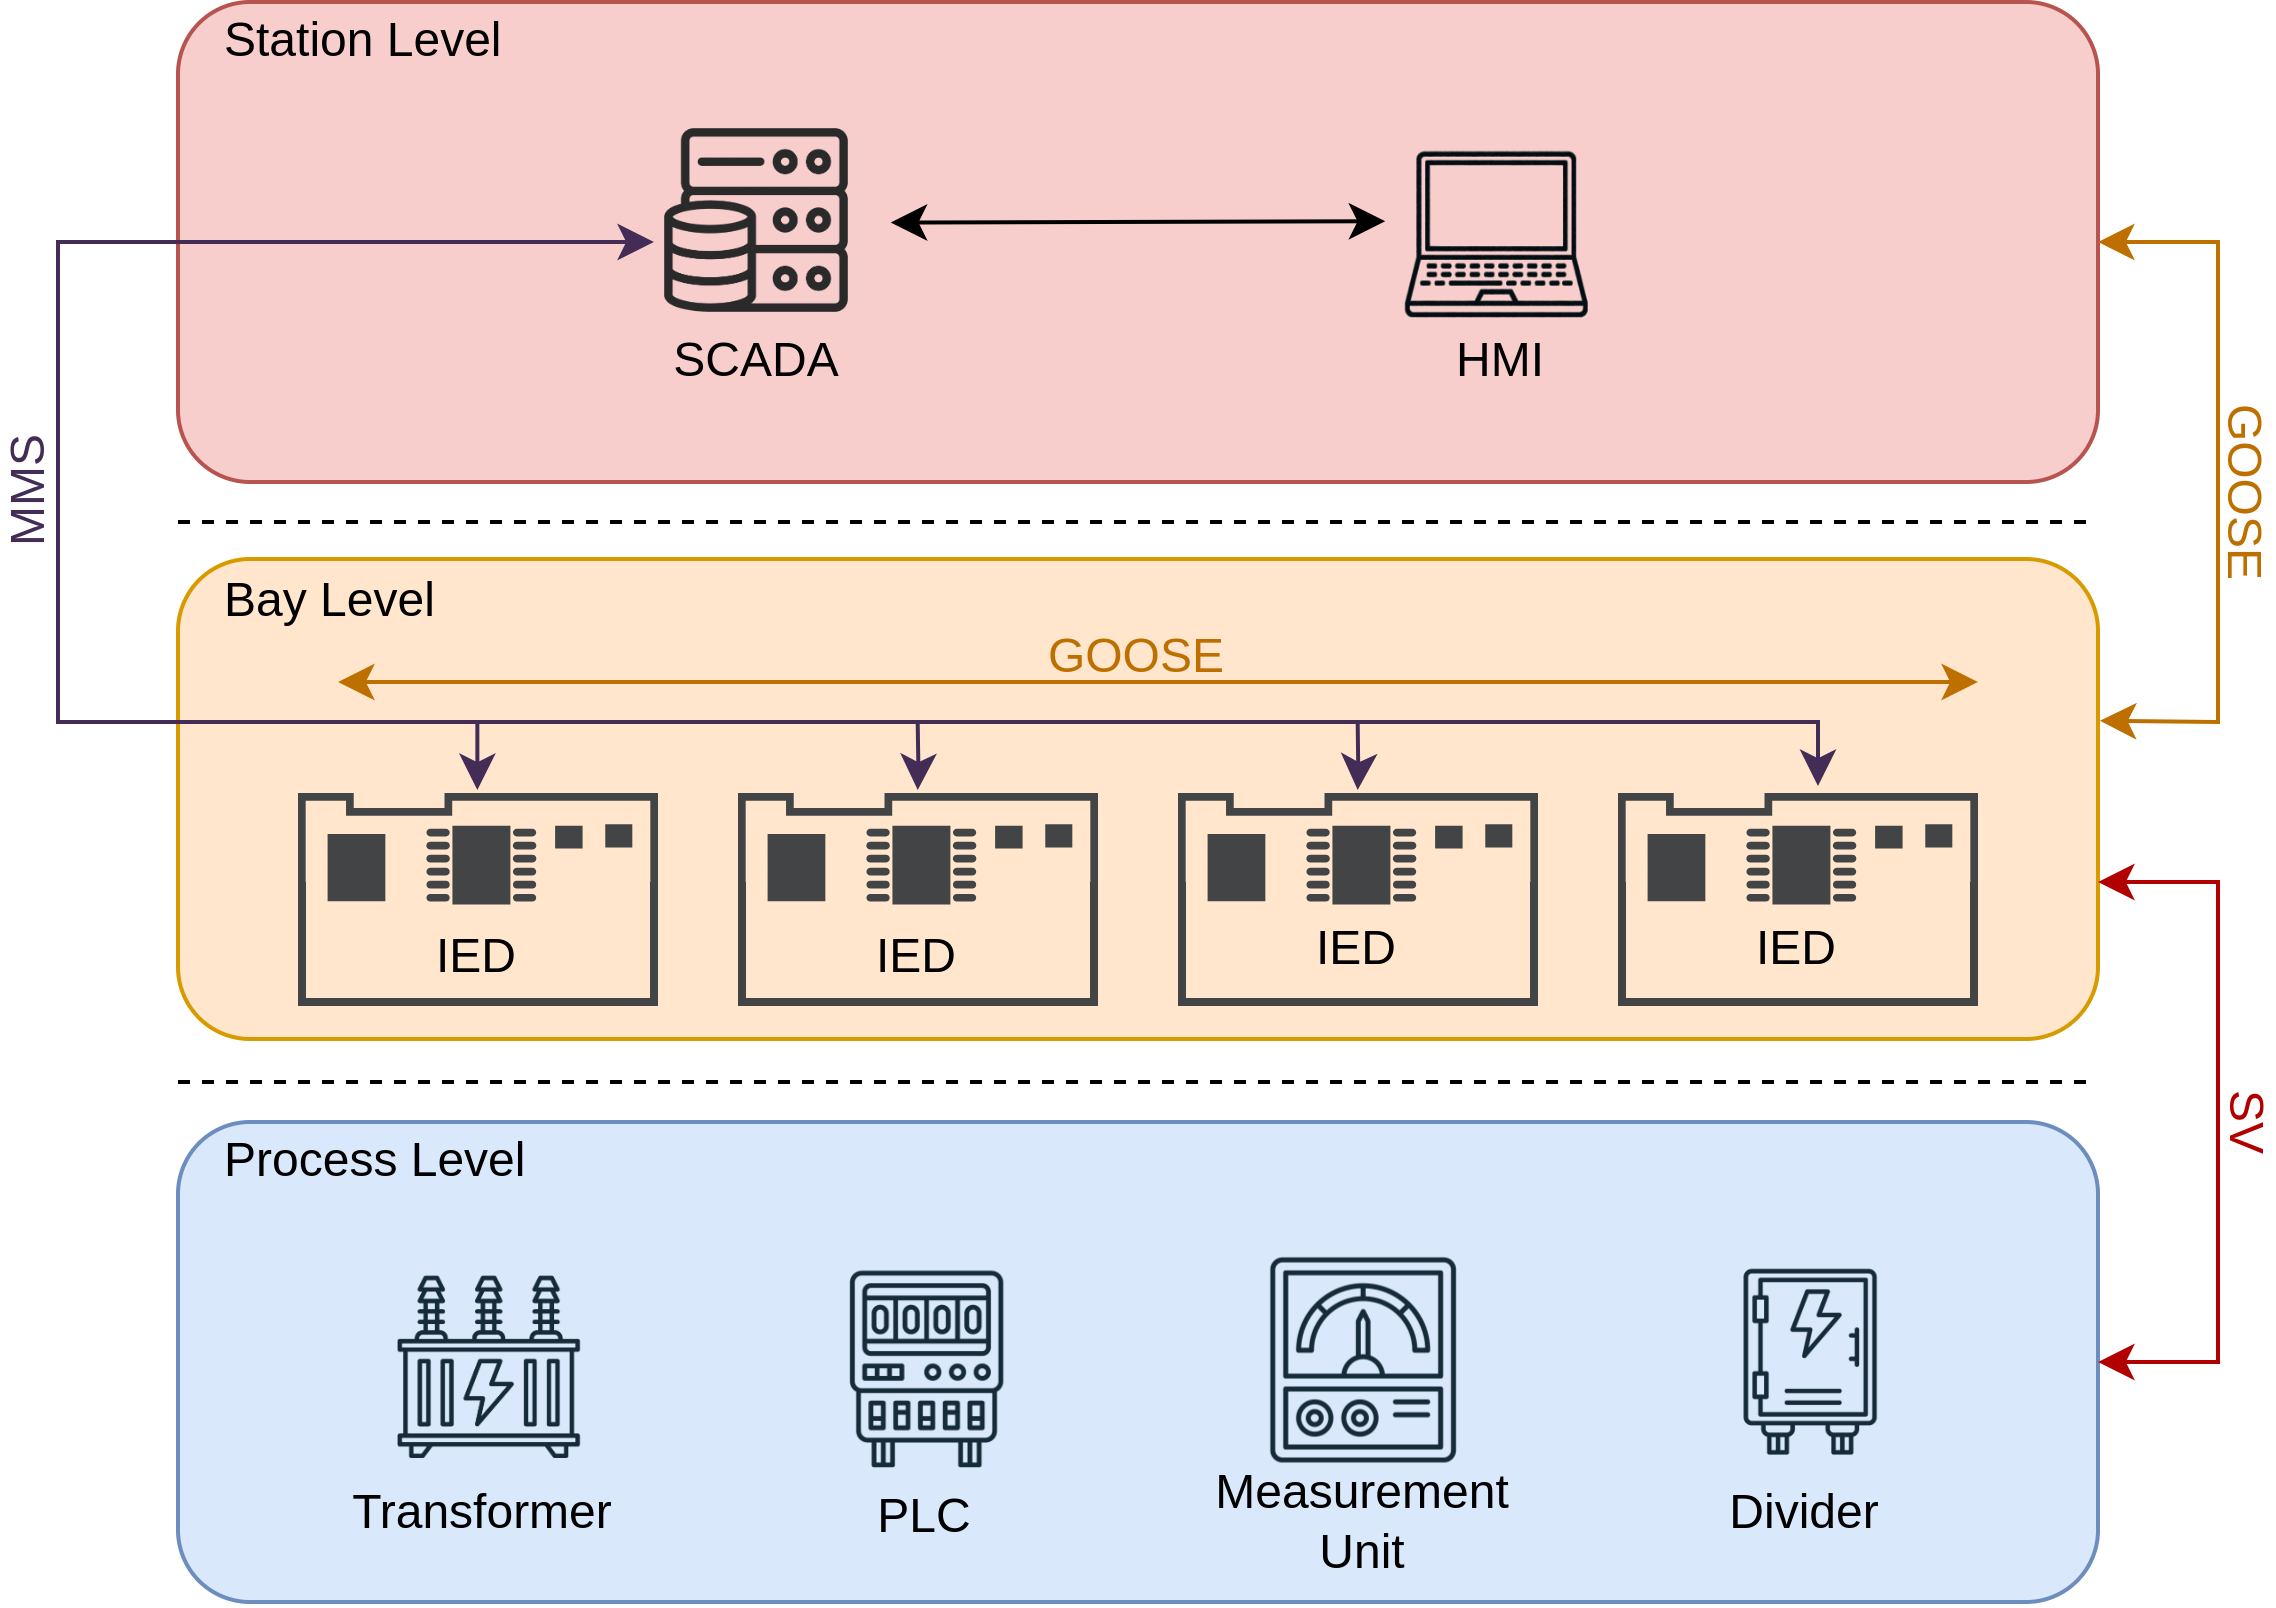
\includegraphics[width=0.45\textwidth]{images/IEC61850_Architecture.png}
    \caption{Overview of the three architecture levels in IEC 61850 \cite{SGRWin_IEC61850Architecture:2021}}
    \label{image:IEC61850Architecture}
\end{figure}

\noindent At the lowest point, the process level contains devices tasked with the actual power management. Examples for these are: transformers, circuit 
breakers, Programmable Logic Controllers (PLCs) and measurement units \cite{SGRWin_IEC61850Architecture:2021}. Upon configuration, Process Level components 
periodically publish measurement information to all subscribing communication partner in the Bay Level via Sampled-Value (SV) packets 
\cite{TyphoonHIL_IEC61850SV:2021}. This communication involves LAN-internal multicast packets, which take place exclusively on the second layer 
(=Data Link Layer) of the Open System Interconnection (OSI) model \cite{TyphoonHIL_IEC61850SV:2021}. 

\smallskip
The Bay Level above contains the Intelligent Electronic Devices (IEDs), each of which represents a transformation field in the substation 
\cite[p. 39]{IEC61850-7-1:2011}. The IEDs gather the measurement data from the process level and initially processes them. The resulting information 
is then communicated through Manufacturing Message Specification (MMS) packets to other IEDs and the Station Level components \cite[p. 44]{IEC61850-8-1:2011}. 
Simultaniously the IEDs receive control signals from the Station Level, which are also transmitted via MMS packets \cite{trafficGen_IEC61850:2011}. 
As the Station Level components are not necessarily located in the same LAN as the IEDs, the MMS messaging is implmented through TCP packets on the 
fourth layer (=Transport Layer) of the OSI model \cite[p. 45]{IEC61850-8-1:2011}. In addition to the MMS messaging, the IEDs use Generic Object 
Oriented Substation Events (GOOSE) to send time-critical information to surrounding IEDs. Simmilar to SV, GOOSE messages are implemented through 
broadcast Ethernet packets in the LAN \cite{GOOSE_confidentiality_integrity:2020}.

\smallskip
The devices located in the Station Level of the architecture are responsible for controlling the SAS. This is achieved through MMS packets adressed 
to specific IEDs and the presentation of the processed information in graphical illustrations to the user \cite{SGRWin_IEC61850Architecture:2021}. 
For this, the Station Level components typically consist of a Supervisory Control and Data Acquisition (SCADA) component and a Human-Machine-Interface 
(HMI). Lastly, as displayed in Figure \ref{image:IEC61850Architecture}, it is possible to transmit GOOSE messages to the Station Level components. 
For this the IEC 61850-90-5 standard \cite{IEC61850-90-5:2012} defines a routable version of the layer two GOOSE frame. For this purpose, the Ethernet 
packets are extended by adding network and transport layer headers to form a UDP packet, which is routable throughout a Wide Area Network (WAN) 
\cite{routable_GOOSE_SV:2020}.

%----------------------------------------------------------------------------------------------------------------------------------------------------%
\subsection{Message Security according to IEC 62351}
\noindent Building on the IEC 61850 message types described in Chapter \ref{subchapter:IEC61850}, the IEC 62351 standard \cite{IEC62351:2024} dictates 
security goals and requirements for cybersecurity solutions. In order to evaluate the proposed MACsec solution for industrial applications correctly, 
we need to assess the proposed security functions according to the demands of this standard.

\smallskip
With regard to MMS messaging, the standard divides the security requirements according to the layers of the OSI reference model. The upper three layers 
are summarized in the application profile and the lower four layers in the transport profile \cite{SecureMMS:2020}. Based on this, the standard specifies 
that the security system shall verify the authenticity of the communication partner and the integrity of the transmitted messages during the handshake 
phase of the transport profile \cite{Review_IEC62351:2019}. Following this the system shall provide confidentiality for the outgoing messages in the 
data transfer phase \cite{SecureMMS:2020}. With respect to the upper three layers, the standard specifies two possible implementations in the application 
profile: peer-to-peer security and End-to-End security \cite{Review_IEC62351:2019}. The primary difference between them consists in the data origin 
authentication and message integrity checks, which are only verified during the association establishment in the peer-to-peer implementation, whereas 
the End-to-End implementation also ensures them in the following data transfer \cite{Review_IEC62351:2019}.

\smallskip
For GOOSE messages the standard argues, that the strict real-time requirement of a maximum of 3 ms \cite{GOOSE_confidentiality_integrity:2020} outweighs 
the safety requirements and for this reason state, that security measures, which affect the trasnmission rates are not acceptable \cite{PoisonedGOOSE:2014}. 
Building on this the IEC 62351 standard advises against the encryption of GOOSE messages and only proposes the use of digital signatures to verify the 
authenticity of the GOOSE publisher and the integrity of the message. As simmilar restrictions arise for SV messages, the standard equally advises the 
usage of digital signatures for SV packets \cite{Review_IEC62351:2019}. 

%----------------------------------------------------------------------------------------------------------------------------------------------------%
\subsection{Fundamentals of the MACsec Security Standard}
\noindent MACsec poses an information security standard, which protects messages on the second layer (=Data Link Layer) of the OSI model. In contrast 
to security standards operating in higher layers of the TCP/IP stack (e.g. Transport Layer Security (TLS)), which provide End-to-end encryption, MACsec 
verifies the integrity and authenticity of a packet within each hop of the transmission \cite{Cybersecurity_Substation:2016}. However, this lower layer 
implementation close to the PHY enables MACsec to secure communication, which takes place exclusively in Ethernet packets (e.g. SV \& GOOSE). The 
following paragraph explains the most important aspects of the MACsec standard, which are responsible for ensuring the authenticity, integrity and 
confidentiality of the transmitted packets.

\begin{figure}[h]
    \centering
    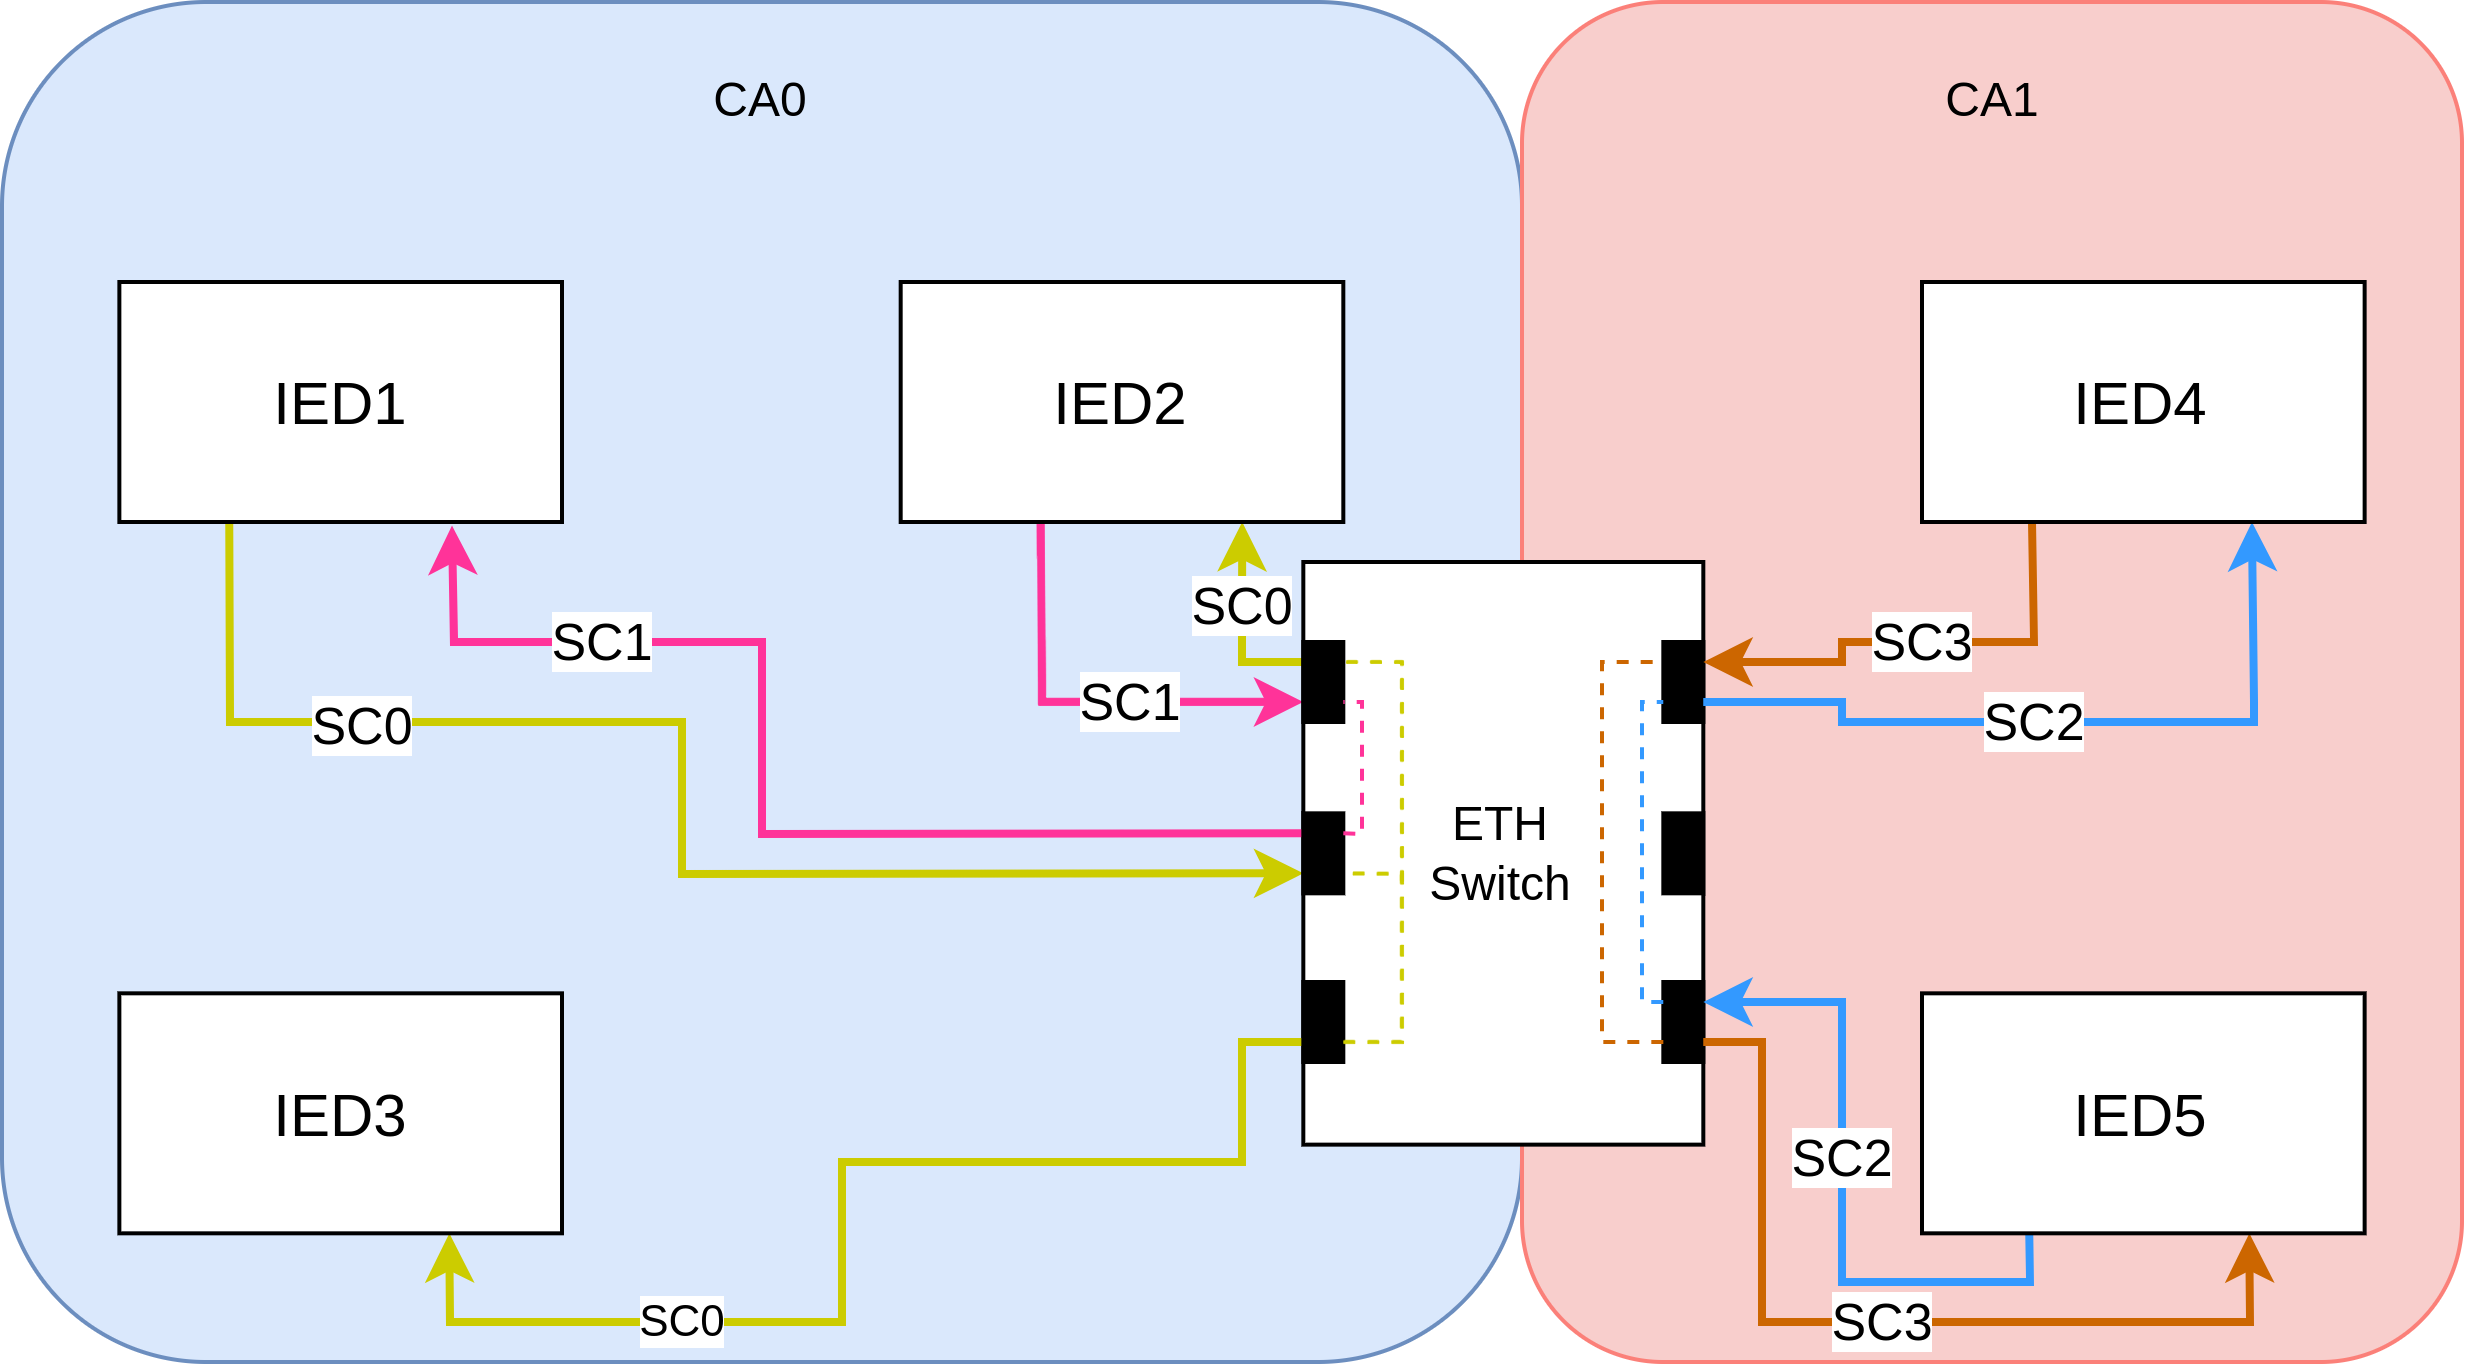
\includegraphics[width=0.45\textwidth]{images/MACsec_Entities_Diagram.png}
    \caption{Schematic representation of the MACsec entities \cite{IEEE-802-1AE:2018}}
    \label{image:MACsecEntities}
\end{figure}

\noindent As displayed in Figure \ref{image:MACsecEntities}, the communicating devices are initially grouped in Connectivity Associations (CAs), which 
represent the logical separation of secured communication areas \cite[p. 35]{IEEE-802-1AE:2018}. Each member of a CA possesses the associated Connectivity 
Association Key (CAK), which is later used to generate the individual session keys. Simmilar to other encryption systems, the CAK acts as a shared 
secret between the individual parties and is therefore used to verify the authenticity of incoming MACsec frames. In the IEEE 802.1AE standard the 
distribution of the CAK among the participants is only specified as a brief overview of the established methods \cite[p. 230]{IEEE-802-1AE:2018}. 
In our case, we utilize pre-shared keys to configure the CA in the test set up explained in chapter \ref{chapter:implementation}.

\smallskip
Within a CA, the connections between the communicating devices are referred to as Secure Channels (SCs). As displayed in Figure \ref{image:MACsecEntities}, 
a SC is a unidirectional connection from a transmitter to one or more receivers. Each SC can be identified by the Secure Channel Identifier (SCI), 
which is added to the MACsec specific field in the secured frame \cite[p. 43]{IEEE-802-1AE:2018}. During transmission on a SC, the packets are sent 
within Security Associations (SAs). These are time intervals in which a single Secure Association Key (SAK) is valid \cite[p. 44]{IEEE-802-1AE:2018}. 
The SAK is the session key, which is derived from the previously described CAK and is only valid for up to ${(2^{32} -1)}$ packets, after which a new 
SAK needs to be generated \cite[p. 66]{IEEE-802-1AE:2018}. To be able to monitor the number of transmitted packets in an SA, the MACsec frame contains 
a packet number field, which is incremented with each subsequent packet. This field aditionally ensures, that no replay attacks can be carried out on 
the network \cite[p. 145]{IEEE-802-1AE:2018}. 

\smallskip
To ensure confidentiality and integrity of the transmitted frames, MACsec utilizes Authenticated Encryption with Associated Data (AEAD) cipher suites. 
These encryption system typically consist of a symmetric block cipher, wich provides the option to encrypt the payload of the message and generates a 
Message Authentication Code (MAC) over the entire message \cite{GOOSE_confidentiality_integrity:2020}. For usage the IEEE 802.1AE standard specifies 
four variations of the Advances Encryption System in Galois/Counter Mode (AES-GCM) \cite[p. 143ff]{IEEE-802-1AE:2018}.

%%%%%%%%%%%%%%%%%%%%%%%%%%%%%%%%%%%%%%%%%%%%%%%%%%%%%%%%%%%%%%        Related Work         %%%%%%%%%%%%%%%%%%%%%%%%%%%%%%%%%%%%%%%%%%%%%%%%%%%%%%%%%%%
\section{Related Work}
\label{chapter:relatedWork}
\noindent To assess the operating principal of a MACsec-based security system in IEC 61850 compliant communication it is necessary to understand both 
the working method of the communication inside a substation as well as the corresponding functionality of the MACsec security standard. The following 
related work display these important aspects and are therefore relevant for the implementation of an experimental set up for MACsec secured industrial 
communication.

\smallskip
Mackiewicz \cite{IEC61850_Overview:2006} describes the overall usage of the IEC 61850 protocol by displaying key features as well as the general aspects 
of IEC 61850 compliant communication. Since this standard represents a core part of the communication inside of power grid systems, it is vital to 
understand the corresponding aspects such as communication paths, model structures or data addressing in order to design a representative test environment. 

\smallskip
Hussain  \textit{et al.} \cite{Review_IEC62351:2019} published a paper assessing the IEC 62351 standard and its security mechanisms towards IEC 61850 
compliant messaging. The publication initially describes the basic values and security goals of the safety standard and, building on this, which attacks 
can potentially be carried out on IEC 61850 messages to manipulate the internal workings of a SAS. At this point the paper primarily focuses on the 
Ethernet-based message types GOOSE and SV and the associated decision not to encrypt them due to strict time delivery requirements.  

\smallskip
Lackorzynski \textit{et al.} \cite{MACsecIndustrialOptimization:2020} proposed modifications of the IEEE 802.1AE standard to improve MACsec for usage 
in industrial applications. In particular, the fragmentation of Ethernet frames was considered. This procedure is necessary, if messages exceed the 
Maximum Transmission Unit (MTU) and are thus possibly discarded by the recipient of the message. The presented implementation ensures this parameter 
and spits messages into multiple frames, if it is exceeded. Additionally the authors discuss the usage of different cipher suits instead of the 
AES-GCM 128/256 specified in the MACsec standard. The evaluation of their study shows that the ChaCha20-Poly1305 cipher is a promising alternative 
for industrial applications.

\smallskip
Moreira \textit{et al.} \cite{Cybersecurity_Substation:2016} evaluate various approaches to introduce cyber security in SASs. Initially, a brief outline 
of the communication structures in substations is presented. Building on this, various established security approaches are explained and evaluated based 
on the protection objectives of the IEC 62351 standard. The authors also point out possible implementation problems, such as incompatibilities between 
the security systems and the communication protocols or the handling of redundant packets inside ring-topology networks. In the further course of the 
paper, they present the idea of MACsec based communication security in SASs and the associated advantages and challenges that arise with it. 

\smallskip
Hussain \textit{et al.} \cite{GOOSE_confidentiality_integrity:2020} analyzed possible GOOSE security implementations based on their preceding review 
of the IEC 62351 standard \cite{Review_IEC62351:2019}. Especially concerning the decision to abstain from implementing confidentiality in GOOSE messages, 
the authors argue, that the critical payload of these messages demand encryption to provide efficient protection against attacks. However, in order to 
meet the real-time requirements of the protocol, they suggest replacing the RSA signature with encryption using an AEAD cipher. In the further course 
of the paper they compare encryption and signature times between different AEAD ciphers and conclude based on the measurement results, that these encryption 
systems pose a promising solution, which provides the opportunity to encrypt the message while simultaniously  meeting the 3 ms timing requirement.

\smallskip 
Building on the theoretical proposition of Moreira \textit{et al.} \cite{Cybersecurity_Substation:2016}, we formulate our evaluation of MACsec carried 
out for use in substations and other power systems based on the IEC 61850 standard. Along with this, we consider the findings of Hussain \textit{et al.} 
\cite{GOOSE_confidentiality_integrity:2020} in relation to the usage of Encrypt-then-MAC AEAD ciphers in the implementation of our MACsec test environment. 
From this, our experimental setup enables us to discuss the advantages and disadvantages of MACsec in comparison with the security goals of the IEC 62351 
standard. 

%%%%%%%%%%%%%%%%%%%%%%%%%%%%%%%%%%%%%%%%%%%%%%%%%%%%%%%%%%%%%%       Implementation        %%%%%%%%%%%%%%%%%%%%%%%%%%%%%%%%%%%%%%%%%%%%%%%%%%%%%%%%%%%
\section{Implementation}
\label{chapter:implementation}
\noindent To test the mode of communication in a SAS, we implement a test environment consisting of three Bay Level components. As the IEDs take part 
in all forms of message exchange inside the Substation Architecture, they are perfectly suitable for testing the communication in conjunction with MACsec. 

\smallskip
In order to ensure the reproducibility of this study, we decided to use the Raspberry Pi 4 as hardware plattform for all devices in the setup. With respect 
to the software used in the applications, we utilize the open source library libiec61850\footnote{source: https://libiec61850.com/} to establish the 
different communication types and data structures of the IEC 61850 standard. To integrate MACsec into the communication, we utilize the MACsec Linux kernel 
module\footnote{source: https://github.com/torvalds/linux/blob/master/drivers/net/macsec.c}, which establishes a configurable virtual interface on top of 
an existing network interface \cite{MACsecLinuxModuleDoc:2016}. For the implementation of time measurement in chapter \ref{subchapter:TestProcedures},  

\smallskip 
The remainder of this chapter is structured as follows: Chapter \ref{subchapter:TestEnvironmentStructure} initially explains the overall structure of the 
test environment. Building on this, Chapter \ref{subchapter:TestEnvironmentMACsec} describes the overall MACsec configuration and the corresponding entities 
of the security standard. Lastly Chapter \ref{subchapter:TestProcedures} elaborates on the subsequent test executions. 

\subsection{Structure of the Test Environment}
\label{subchapter:TestEnvironmentStructure}
\noindent As displayed in Figure \ref{image:MACsecTestSetup}, we configure IED1 as a publishing server and IED2 and IED3 as communication clients. 
Furthermore the implementation of IED1 contains a XML data structure compliant to the specification of the Substation Configuration Language (SCL) 
in IEC 61850-6 \cite{IEC61850-6:2010}. This file contains the communication and processing information of the IED itself \cite{IEC61850_Overview:2006}.

\smallskip
In our case, we integrated a measurement unit (MMXU) \cite[p. 268]{IEC61850-7-4:2010} and a control unit (LLN0) \cite[p. 164]{IEC61850-7-4:2010} 
into the SCL file. During runtime, IED1 continuously populates the data points of the measuring unit with sampled values of a sinusoidal function. In 
addition to the actual measurement, each sampled value contains a time stamp and a quality index \cite[p. 61ff]{IEC61850-7-3:2010}. These values can 
then be requested by IED2 and IED3 via MMS messages.

\begin{figure}[h]
    \centering
    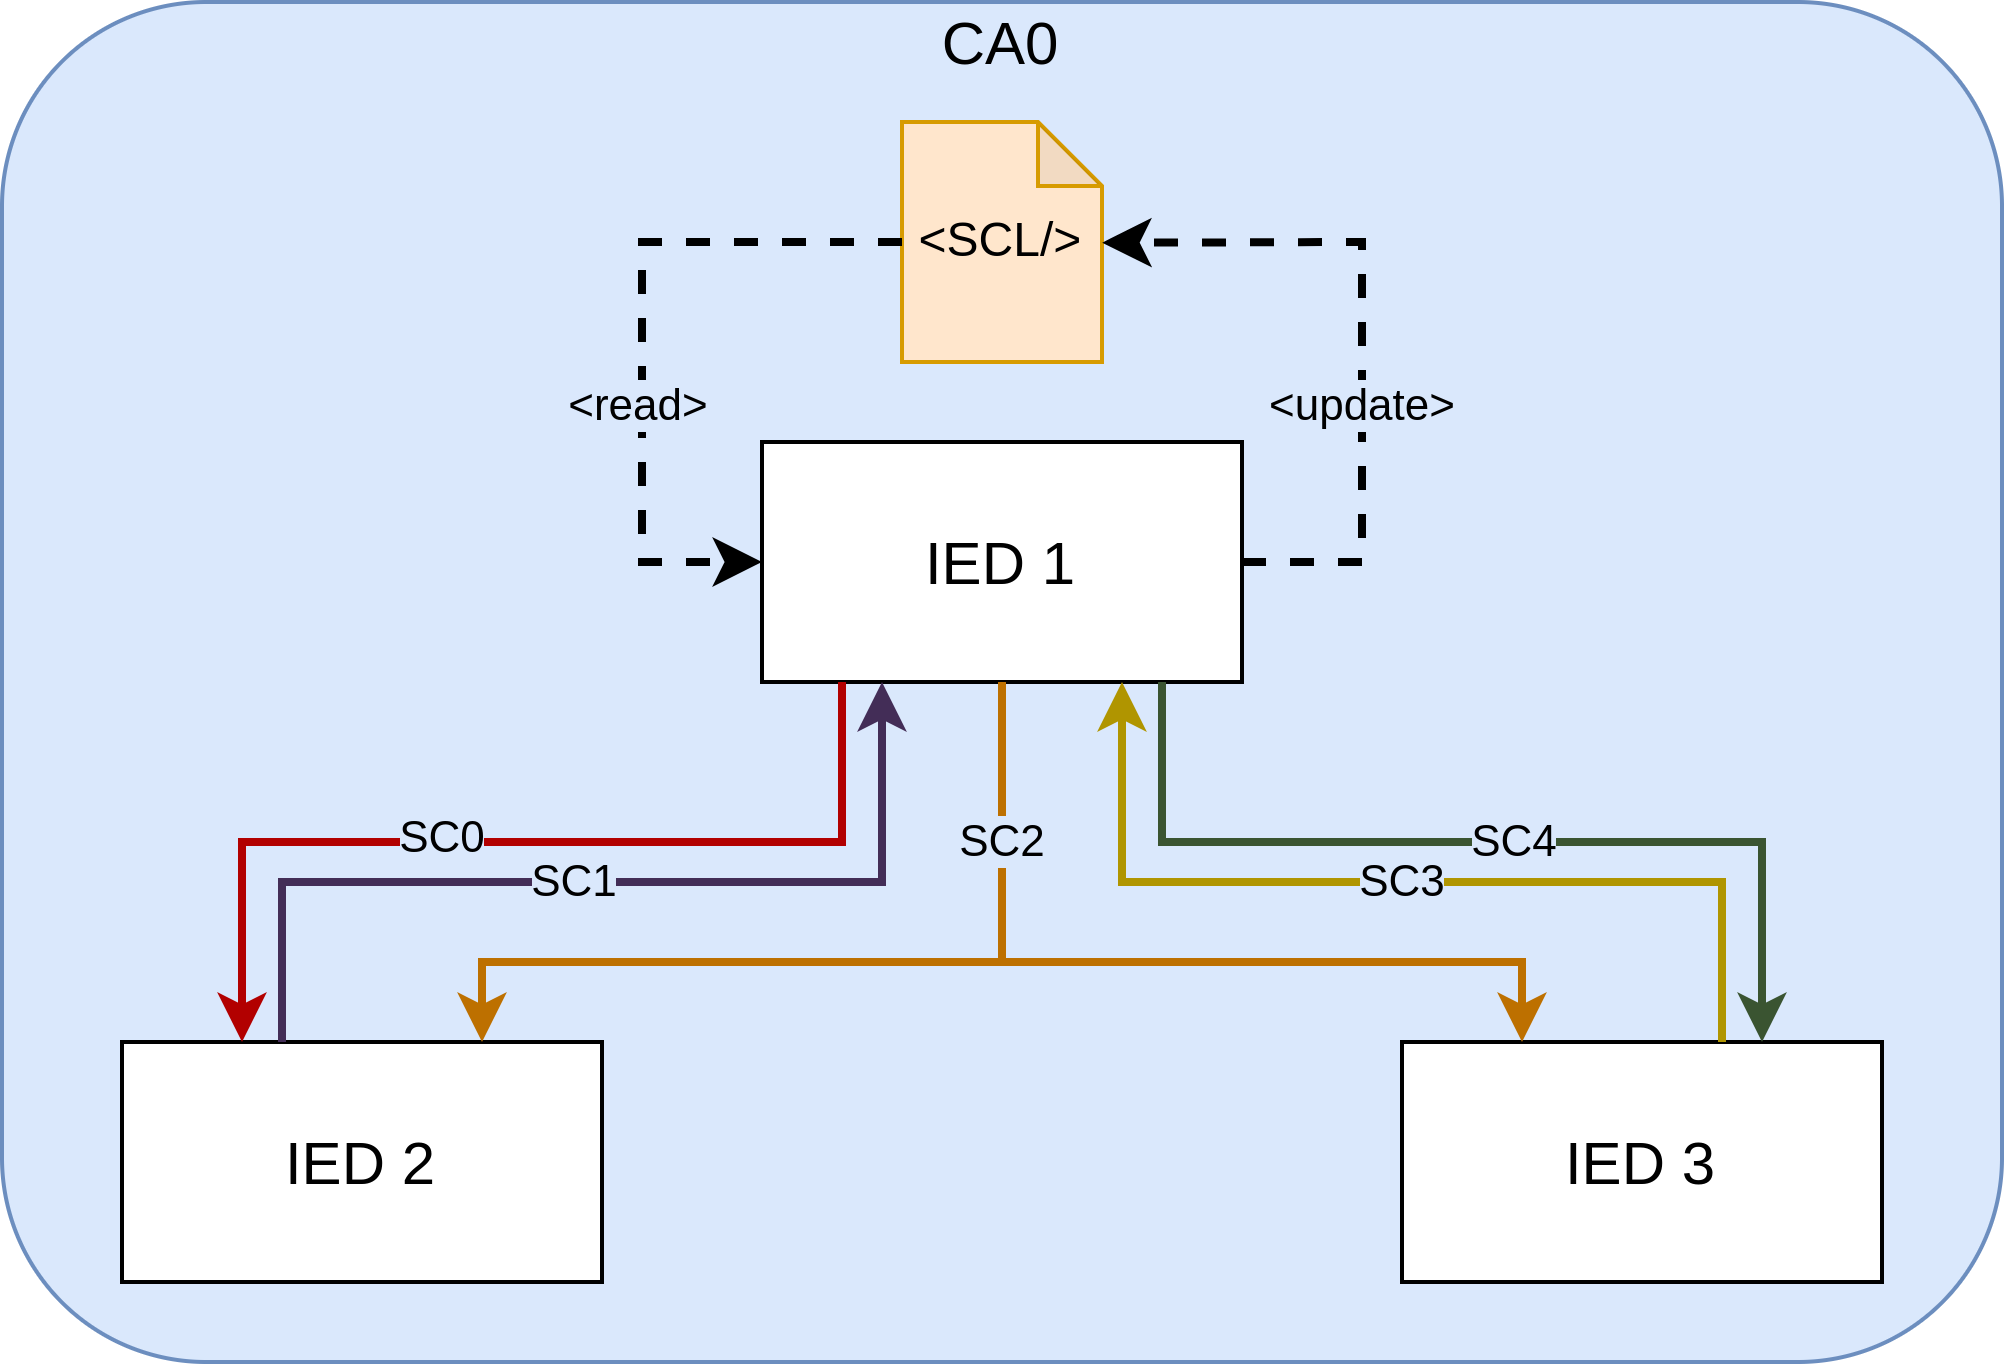
\includegraphics[width=0.45\textwidth]{images/TestSetupIEDs.png}
    \caption{Component Structure of the Test Setup}
    \label{image:MACsecTestSetup}
\end{figure}

\noindent In addition to the TCP request-response communication via MMS messages, IED1 periodically publishes GOOSE messages in a configurable interval 
containing the current value of the measurement. The configuration of the GOOSE messages, which contain the corresponding broadcast MAC address, VLAN 
Id and VLAN priority are equally stored in the control unit of the SCL file \cite[p. 189]{IEC61850-8-1:2011}. On the client side, the subscription to 
the corresponding events is implemented in software, subsequently resulting in a logging function, which provides the latest information. 

%----------------------------------------------------------------------------------------------------------------------------------------------------%
\subsection{MACsec integration in the Test Environment}
\label{subchapter:TestEnvironmentMACsec}
\noindent Building on the general structure described in chapter \ref{subchapter:TestEnvironmentStructure}, the implementation of MACsec into the test 
setup can now be explained. In doing so, we primarily integrated all devices in the same CA by distributing a pre-shared CAK. Based on this key, the 
various SCs and SAs can be established as shown in Figure \ref{image:MACsecTestSetup}.

\smallskip
For bidirectional MMS communication between two IEDs, one SC is required for each communication direction. Using the example of packet exchange between 
IED1 and IED2, we have configured the secure channels SC1 and SC2 for this purpose. Each of these channels derives its own SAK from the CAK and 
establishes a secure connection for the duration of the SA. The establishment of SC3 and SC4 is carried out identically for MMS communication between 
IED1 and IED3.

\smallskip
With regard to the secure publication of GOOSE we established an additional SC (displayed in Figure \ref{image:MACsecTestSetup} as SC2), which is 
connected to both IED2 and IED3. This configuration enables us to broadcast the message while simultaniously securing the payload and ensuring 
authenticity and integrity of the package.  

%----------------------------------------------------------------------------------------------------------------------------------------------------%
\subsection{Definition of the Test Procedures}
\label{subchapter:TestProcedures}
\noindent To evaluate whether this MACsec implementation fulfills the requirements of the IEC 62351 standard, we conduct a measurement of the 
transmission times for each of the different package types. In order to achieve a precise time measurement, we expanded the implementation of the server 
and the client application to toggle a General Purpose Input/Output (GPIO) pin during transmission and reception of the associated frame. 

\smallskip
By using an external logic analyzer, the times between the voltage level shifts can be measured in the next step. Since the measurement is performed by 
an external device, we do not need clock synchronization between the communication participants.

%%%%%%%%%%%%%%%%%%%%%%%%%%%%%%%%%%%%%%%%%%%%%%%%%%%%%%%%%%%%%%         Evaluation          %%%%%%%%%%%%%%%%%%%%%%%%%%%%%%%%%%%%%%%%%%%%%%%%%%%%%%%%%%%
\section{Evaluation}
\label{chapter:evaluation}


%%%%%%%%%%%%%%%%%%%%%%%%%%%%%%%%%%%%%%%%%%%%%%%%%%%%%%%%%%%%%%         Conclusion          %%%%%%%%%%%%%%%%%%%%%%%%%%%%%%%%%%%%%%%%%%%%%%%%%%%%%%%%%%%
\section{Conclusion}
\label{chapter:conclusion}


%%%%%%%%%%%%%%%%%%%%%%%%%%%%%%%%%%%%%%%%%%%%%%%%%%%%%%%%%%%%%%     Begin of References      %%%%%%%%%%%%%%%%%%%%%%%%%%%%%%%%%%%%%%%%%%%%%%%%%%%%%%%%%%
\printbibliography

%%%%%%%%%%%%%%%%%%%%%%%%%%%%%%%%%%%%%%%%%%%%%%%%%%%%%%%%%%%%%%%%%%%%%%%%%%%%%%%%%%%%%%%%%%%%%%%%%%%%%%%%%%%%%%%%%%%%%%%%%%%%%%%%%%%%%%%%%%%%%%%%%%%%%%
\end{document}
